% TO DO:
% Plot catalog (histogram and sample sky)
% Select brightess sources
% Principle component analysis???!!!!

% Introduction
% add coverage plot
% finish ubercal in matrix form

%% Use whichever is most appropriate for your purposes.
%%
%%\documentclass[12pt,preprint]{aastex}
%% manuscript produces a one-column, double-spaced document:
\documentclass[manuscript]{aastex}
%% preprint2 produces a double-column, single-spaced document:
%% \documentclass[preprint2]{aastex}

%% Sometimes a paper's abstract is too long to fit on the
%% title page in preprint2 mode. When that is the case,
%% use the longabstract style option.

%% \documentclass[preprint2,longabstract]{aastex}


\newcommand{\vdag}{(v)^\dagger}
\newcommand{\myemail}{holmes@mpia.de}
\newcommand{\true}{\mathrm{true}}

%% You can insert a short comment on the title page using the command below.

\slugcomment{Version 0.1}

\shorttitle{Optimizing Large Scale Surveys for Photometric Calibration}
\shortauthors{Holmes et al.}

\begin{document}

%% LaTeX will automatically break titles if they run longer than
%% one line. However, you may use \\ to force a line break if
%% you desire.

\title{Optimizing Large Scale Surveys for Photometric Calibration, \\
    The Euclid Dark Energy Mission as an Example}

%% Use \author, \affil, and the \and command to format
%% author and affiliation information.
%% Note that \email has replaced the old \authoremail command
%% from AASTeX v4.0. You can use \email to mark an email address
%% anywhere in the paper, not just in the front matter.
%% As in the title, use \\ to force line breaks.

\author{Rory Holmes\altaffilmark{1}, David W. Hogg\altaffilmark{1,2} and H.-W. Rix\altaffilmark{1}}

%% Notice that each of these authors has alternate affiliations, which
%% are identified by the \altaffilmark after each name.  Specify alternate
%% affiliation information with \altaffiltext, with one command per each
%% affiliation.

\altaffiltext{1}{Max-Planck-Institut f\"ur Astronomie, K\"onigstuhl 17, Heidelberg, 69117, Germany.}
\altaffiltext{2}{Center for Cosmology and Particle Physics, Department of Physics, New York University, 4 Washington Place, New York, NY 10003, USA.}

%% Mark off your abstract in the ``abstract'' environment. In the manuscript
%% style, abstract will output a Received/Accepted line after the
%% title and affiliation information. No date will appear since the author
%% does not have this information. The dates will be filled in by the
%% editorial office after submission.

\begin{abstract}
XX
\end{abstract}

%% Keywords should appear after the \end{abstract} command. The uncommented
%% example has been keyed in ApJ style. See the instructions to authors
%% for the journal to which you are submitting your paper to determine
%% what keyword punctuation is appropriate.

\keywords{XX, XX, XX}

\section{Introduction}
Astronomers tend to think in terms of taking science data and calibration data separately. The former is used for science and the latter is used to set instrument parameters like flat-field, bias and so-on. But typically far more photons are collected during science exposures; are these not incredibly constraining on the calibration themselves? Indeed, in the retrospective photometric calibration of the Sloan Digital Sky Survey data (XX ref) (SDSS) much more calibration information was obtained from the science data than the calibration data. But, of course, the SDSS imaging strategy had to be adjusted to make this calibration work: good redundancy is required in the data stream, and a redundancy of a very specific kind.

In this paper we will show that this distinction between science and calibration data no longer applies in the large survey mission, both ground and space based, currently being planned and developed. We show that, as long as the survey strategy is designed appropriately, the calibration information within the science data can be used to accurately constrain the relative photometric response of an imaging instrument. This retrospective, cross-calibration of the dataset is a very powerful calibration method; future large scale imaging surveys should be optimized with this in mind. 

We concentrate on catalog level simulations of different survey strategies and assess how well the resultant dataset can be used to constrain the relative response of the imaging instrument it came from. Although we do not model the imaging instrument on a pixel scale, we do include realistic measurement uncertainties within the simulations. 

Although the results we present here are general to all large scale imaging surveys, in Section XX we focus on the proposed Euclid Deep Field Survey. This survey has been optimized, within other constraints, based on the results from this work. 

\section{Simulating the Measured Source Database}
To assess how well this cross-calibration performs with different observation strategies, we first constructed the required simulation machinery to take an observing strategy as an input, generate a realistic sky, perform the survey - with appropriate measurement uncertainties - and cross-calibration the resulting dataset. The following subsections detail the main methods and assumptions used in our simulations.  

\subsection{Sky Catalog}
We first create a catalog of fake sources, both stars and galaxies, based on realistic densities within the magnitude range $m_{min} < m < m_{max}$. We choose these limits based on the properties of single exposure of the current configuration of Euclid NIR Imaging Channel (NIP): $m_{min} = 17$, the approximate saturation limit, and $m_{max} = 22$, the 10$\sigma$ limit. Sources are generated with random coordinates (uniformly distributed within the sky region being investigated) and with random magnitudes distributed according to the following powerlaw:
\begin{displaymath}
\log_{10} \frac{dN}{d\Omega\,dm} = a + b\,m
\end{displaymath}
Where $a$ sets the total source density and $b_{star} = 0.25$ steller and galaxy populations reported in XX. We make no distinction between stars and galaxies in our simulations. The random number generator is given the same seed, so that the same simulated sky is produced each time the simulation is run. This ensures that the differences observed are not a result of random fluctuations. We relate source magnitudes, $m$, to source fluxes, $s$, simply by: $m = 22.5 - 2.5\log_{10}(s)$, where the 22.5 puts the fluxes in units of nanomaggies. 

\begin{figure}[ht]
\begin{center}
\includegraphics[width=\textwidth]{temp.png}
\end{center}
\caption{An example catalog of fake sources used within the simulations. The sources are shown at their position on a portion of the sky (left) and as a histogram of their magnitudes (right).
\label{fig:sky}}
\end{figure}

\subsection{Single Exposure}
With a given camera pointing $(\alpha, \beta)$ and camera orientation $(\theta)$, we transform the we transform the sky catalog into focal plane coordinates and find all the stars falling within the instrument's field-of-view. For the instrument's field-of-view, we use the current size of the Euclid NIR imager's: $0.7 \times 0.7$~deg$^{2}$. We do not simulate images, instead we trivially convert the true source fluxes into measured counts $(c)$ with an instrument response model $(f)$ and a measurement uncertainty model. A typical exposure is depicted in Figure \ref{fig:camera}.

\begin{figure}[ht]
\begin{center}
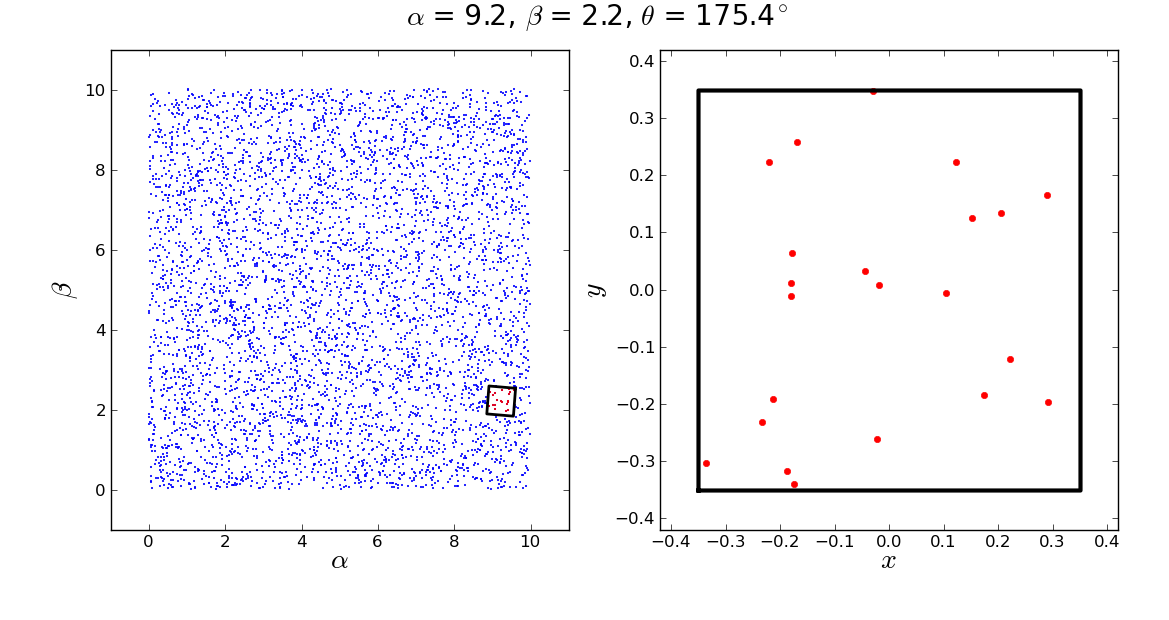
\includegraphics[width=\textwidth]{camera_image.png}
\end{center}
\caption{A single exposure of the fake sky. Left: Plot of the entire fake sky, with the instrument's field-of-view shown. Right: The resultant distribution of the highlighted sources on the instrument's focal plane. \label{fig:camera}}
\end{figure}

\subsubsection{Measurement Model}
For a measurement $i$ the counts recorded from a source $k$ depends on true instrument response $f_{\true}$, which is a function of focal plane position $\vec{x_i}$, and the source's true flux $s$: 

\begin{displaymath}
c_i = f_{\true}(\vec{x_i}) \, s_{k, \true} + e_{i}
\end{displaymath}

\noindent{}An error, drawn from the Normal Distribution $N(e|0,{\sigma_\true}^2)$, is also introduced to the measurement. In this analysis, we do not consider temporal variations in the instrument's response. 

\subsubsection{Noise Model}
\label{sec:noise_model}
We assume that the Euclid exposures will be background limited and that, for systematic reasons, we will hit an upper limit on the signal-to-noise for bright sources. We complicate the model by applying an extra term to the count's uncertainty variance, which we do not take into account in our analysis:
\begin{displaymath}
\sigma_{i, \true}^{2} = (1 + \epsilon_k) \, \alpha^{2} + \eta^{2}\, [ f_\true(\vec{x_i}) \, s_{k, \true} ]^2
\end{displaymath}
\noindent{}where $\epsilon$ is a random number, in the range [0.0, $\epsilon_{max}$), generated for each measurement $i$. 

We do not take into account this final term in our analysis and we therefoer assume that the uncertainty variance on the counts are:
\begin{displaymath}
\sigma_{{i}}^{2} = \alpha^{2} + \eta^{2}\, c^{2}_i
\end{displaymath}
\noindent{}where $\alpha$ and $\eta$ are both constants. In fact, we complicate the model by applying an extra term to the count's uncertainty variance, which we do not take into account in our analysis: 

An example of the assumed compared to the true uncertainty variances is shown in Fig. \ref{fig:invvar}.

\begin{figure}[ht]
\begin{center}
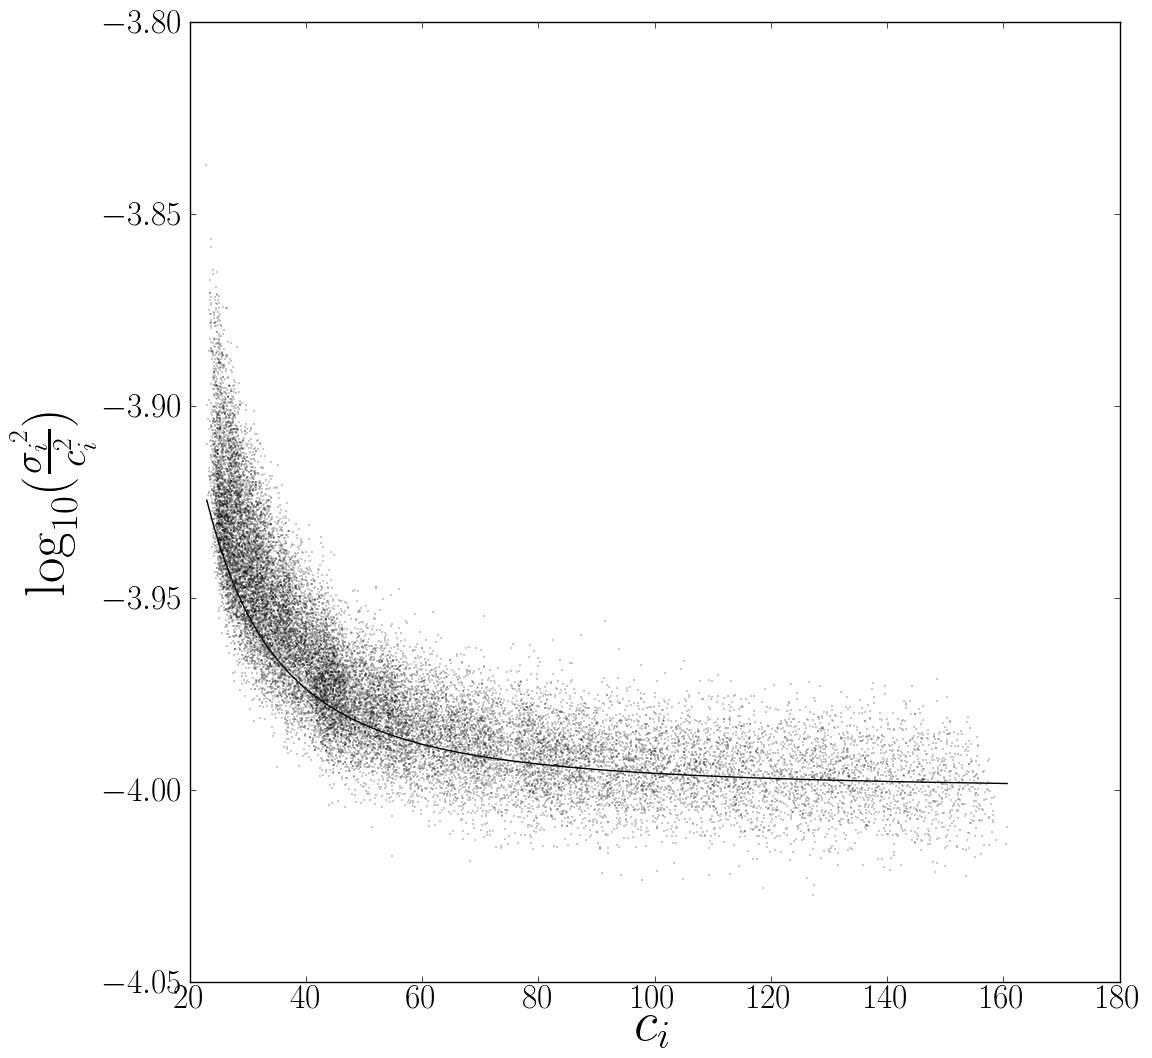
\includegraphics[width=\textwidth]{invvar.png}
\end{center}
\caption{This plot highlights the difference between the assumed (solid line) and the actual (black points) measurement uncertainty variances.\label{fig:invvar}.}
\end{figure}

\subsubsection{Instrument Response Model}
We simulate the instrument response $f_\true(\vec{x_i} | \vec{q}_{\true})$ variations on both large and small scales. We model large scale structure, such as the residual from a flat-field calibration source, as a second order polynomial. We model small scale variations in the instrument response with XX sine and cosine contributions. We intentionally do not for the instrument response with a model of the same form.

\subsection{Cross-Calibrating the Source Dataset}
The next step is to calibrate the simulated dataset generated for the survey being investigated. We consider the same cross-calibration procedure used with a number of ground based surveys, such as SDSS XX. This cross-calibration, termed ``ubercalibration´´ in SDSS terminology is an iterative procedure with two sub-steps: (i) the source fluxes are refined based on the latest instrument response estimate (\textit{s\_step}) and (ii) the instrument response is then refined based on the latest star flux estimates (\textit{q\_step}). We iterate these steps until the solution converges. There is a degeneracy in the problem, as both the true value of the instrument response and the source magnitudes are unknown. With this method we are therefore only able to constrain the relative instrument response. We could not, for example, know if the sources are fainter or if the instrument response is lower. This is not an issue though, as absolute standards are always used to constrain the absolute instrument response. We define a relative instrument response with a set of parameters $\vec{q}$. The individual source measurements are defined as $c_i$ (``counts''), where each $i$ corresponds to a exposure number $n$, a specific star ($k$) and a focal plane position $\vec{x}$.

\noindent{}We solve for the following \textit{incomplete} (see Section \ref{sec:noise_model}) model.
\begin{displaymath}
c_i = f(\vec{x_i} | \vec{q}) . s_{k} + e_{i}
\end{displaymath}
where $s_k$ is a model flux for source $k$ and the error $e_i$ is drawn from the Normal Distribution $N(e|0,{\sigma_i}^2)$. We model the instrument response as a XX order polynominal. 

\noindent{}The two steps in the cross-calibration procedure, called the \textit{s\_step} and the \textit{q\_step}, are detailed in the following two sections:

\subsubsection{Source Flux Refinement (\textit{s\_step})}
The model fluxes of each source, $s_k$, are considered individually. At each \textit{s\_step} we can refine a sources's flux estimate by minimizing the error function with the latest instrument response parameters:

\begin{displaymath}
\chi^2_{k} = \sum_{i \in \mathcal{O}(k)} \frac{(c_i-f_{i}s_{k})^2}{{\sigma_i}^2}
\end{displaymath}

\begin{displaymath}
\frac{d\chi^2_{k}}{d s_{k}} = \sum_{i \in \mathcal{O}(k)} \frac{-2 f_{i} (c_i-f_{i}s_{k+1})}{{\sigma_i}^2} = 0
\end{displaymath}

\begin{displaymath}
s'_{k} \leftarrow \left[{\sum_{i \in \mathcal{O}(k)}  \frac{f_{i}^2}{{\sigma_i}^2}} \right]^{-1}  \left[ {\sum_{i \in \mathcal{O}(k)} \frac{f_{i} c_i}{{\sigma_i}^2}} \right]
\end{displaymath}

The standard uncertainty variance on the new star flux estimate, $s'_{k}$, is given by:

\begin{displaymath}
\sigma'^2_k = \left[{\sum_{i \in \mathcal{O}(k)}  \frac{f_{i}^2}{{\sigma_i}^2}} \right]
\end{displaymath}


\subsubsection{Instrument Response Refinement (\textit{p\_step})}
The instrument response parameters can now be refined with the latest star flux estimates. To do this we minimize the total error function for all measurements with respect to the instrument response parameters.

\begin{displaymath}
\chi^2 = \sum_{k} \chi^2_k
\end{displaymath}
where:
\begin{displaymath}
\chi^2_k = \sum_{i} \frac{(c_i-f_{i}s'_{k})^2}{{\sigma_i}^2}
\end{displaymath}
The instrument response $f_i$ is parameterized as:
\begin{displaymath}
f_{i} = \sum_{l = 1}^L q_{lj} g_l(\vec{x_i})
\end{displaymath}
So the total error function can be rewritten as:
\begin{displaymath}
\chi^2 = \sum_{i} \frac{(c_i- s'_{k} \sum_{l = 1}^L q_{lj} g_l(\vec{x_i}))^2}{{\sigma_i}^2}
\end{displaymath}
The error function is the minimized with respect to the instrument response parameters $q_{lj}$:
\begin{displaymath}
\frac{d\chi^2}{dq_{lj}} = \sum_{i} \frac{-2 g_l(\vec{x_i}) s'_{k} (c_i- s'_{k} \sum_{l' = 1}^{L'} q_{l'} g_{l'}(\vec{x_i}))}{{\sigma_i}^2} = 0
\end{displaymath}

\begin{displaymath}
\sum_{i} \frac{g_l(\vec{x_i}) s'_{k} c_i}{{\sigma_i}^2} = \sum_{i} \frac{g_l (\vec{x_i}) s'^2_{k} \sum_{l' = 1}^{L'} q_{l'} g_{l'} (\vec{x_i})} {{\sigma_i}^2}
\end{displaymath}

These two steps are iterated until the solution converges, or until, it is clear that a solution will not be found. 

\subsubsection{Badness}
To assess the performance of the cross-calibration procedure we define a ``badness'' quantity, which quantifies the difference between the true and fitted instrument response in single number. The focal plane is sampled on a $300 \times 300$ grid and the badness is defined as the root-mean-squared difference between the true and fitted instrument response at these positions. This provides a more complete description of the cross-calibration performance than the RMS of the fitted star fluxes, especially in the case - such as Euclid - in which repeat observations of a deep field will be used to calibrate a wide survey.

\section{Results}
\subsection{Simple Survey Strategies}
In this section we consider four simple, very different, survey strategies. We investigate how well the cross-calibration procedure can constrain the relative instrument response with these surveys. We label these strategies A to D. The different strategies are summarized in Tab. \ref{tab:surveys} and are shown in Fig. \ref{fig:surveys}. Strategy A is the simplest strategy; the field is regularly tiled with a small (XX\%) overlap between adjacent pointings. The pointings in the 12 passes over the same field are exactly aligned. Survey B is the same as A, but with each pass over the field the orientation of the telescope is rotated by $30^\circ$. Survey C is more complex. The first pass over the field is the same as in Survey A, with $12 \times 12$ pointings. In the next pass, one of the pointings in the $\alpha$ directions is removed and one is added in the $\beta$, so our grid of pointings is now $13 \times 11$. The overlap in now XX\% and XX\% in the $\alpha$ and $\beta$ directions respectively. In the third pass over the field, the change to the point grid, compared to the first pass, is reversed and we image the field on a $11 \times 13$ grid. These three passes are then repeated four times. Survey D is quasi-random. The orientation of each pointing is random. The pointing positions are quasi-random: the pointing center is randomly assigned within a $0.7 \times 0.7$ box whose center lies on the pointing grid in Survey A. This is done to ensure a uniform coverage of the field.

\begin{table}
\begin{tabular}{|c|p{5.5cm}|p{3cm}|p{3cm}|}
\hline \textbf{Survey Name} & \textbf{Pointing Center} & \textbf{Pointing Orientation} & \textbf{Number of Pointings}\\ 
\hline \textbf{A} & Uniform Grid ($12\times12$) & Constant & 1728\\ 
\hline \textbf{B} & Uniform Grid ($12\times12$) & 30$^\circ$ Rotation Between Passes & 1728 \\ 
\hline \textbf{C} & Pass 1:  Uniform Grid ($12\times12$) Pass 2:  Uniform Grid ($1§\times11$) Pass 3:  Uniform Grid ($13\times11$)& Constant & 1720 \\ 
\hline \textbf{D} & Quasi-random & Random & 1728 \\ 
\hline 
\end{tabular}   
\caption{A summary of the four simple survey strategies investigated.\label{tab:surveys}}
\end{table}

\begin{figure}[ht]
\begin{center}
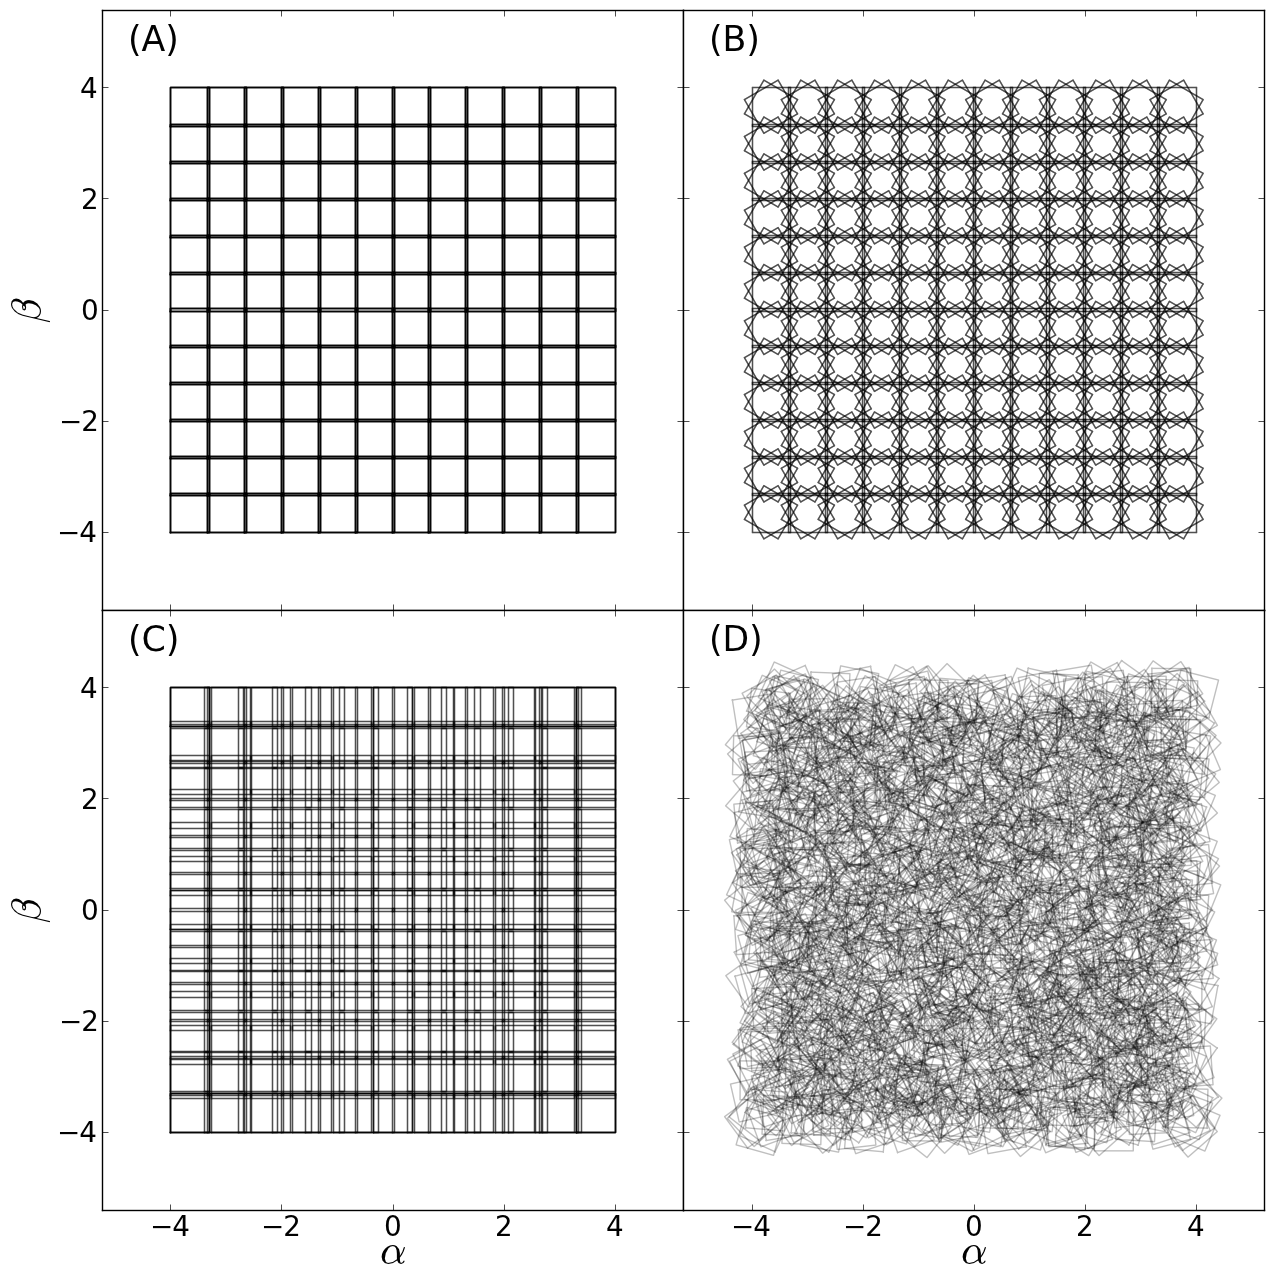
\includegraphics[width=\textwidth]{simple_surveys.png}
\end{center}
\caption{The four simple survey strategies described in the text and summarized in Tab. \ref{tab:surveys}. Surveys A, B and D have 1728 pointings and survey C has 1720 pointings.\label{fig:surveys}}
\end{figure}

\begin{table}
\begin{tabular}{|c|p{4cm}|c|c|}
\hline Survey & Number of Iterations Until Converges & Instrument Response Fit Badness & RMS Source Error \\ 
\hline A & no convergence & - & - \\ 
\hline B & no converges & - & - \\ 
\hline C &  &  &  \\ 
\hline D &  &  &  \\ 
\hline 
\end{tabular}
\caption{The performance of the cross-calibration of the datasets with the survey strategies detailed in Tab. \ref{tab:surveys}\label{fig:simple_results}}
\end{table} 

The difference between the performance of the cross-calibration between Surveys A and B and Surveys C and D is striking. With the former, the solution does not converge. With the later, a fit to the relative instrument response is found after a small number of iterations XX. In both cases, the cross-calibration procedure is able to reproduce the actual instrument response to a high accuracy, with Survey D performing slightly better. 

We can draw a strong conclusion from these simple survey strategies: small and regular overlaps between adjacent pointings is essentially useless for this kind of cross-calibration. The simple strategies, where the sky is just tiled, should be avoided in large scale imaging surveys.



\begin{figure}[ht]
\begin{center}
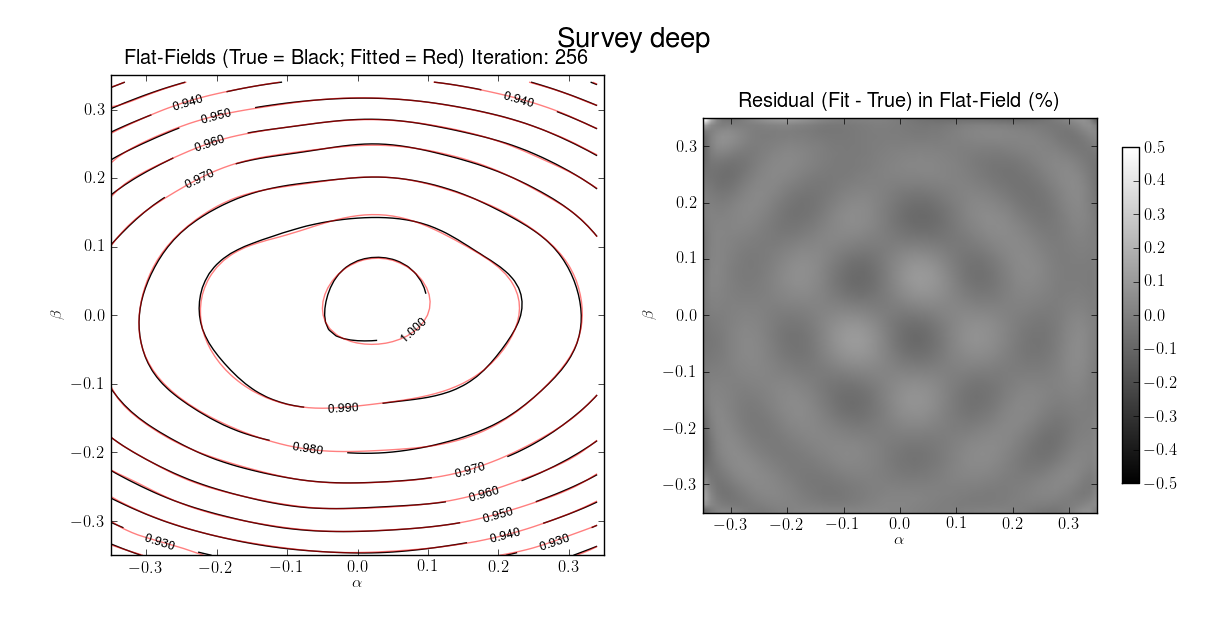
\includegraphics[width=\textwidth]{fit_example.png}
\end{center}
\caption{The fitted flat field compared to the actual flat field found with Strategy D. \label{fig:D}}
\end{figure}


\begin{figure}[ht]
\begin{center}
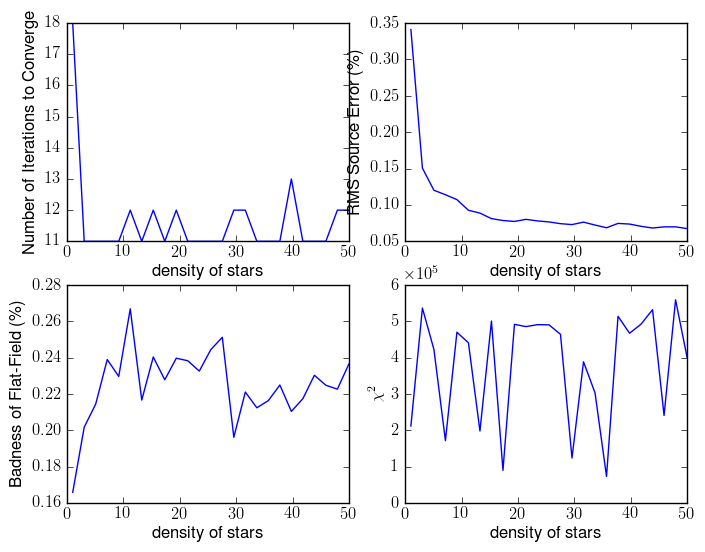
\includegraphics[width=\textwidth]{density_of_stars.png}
\end{center}

\end{figure}


\begin{figure}[ht]
\begin{center}
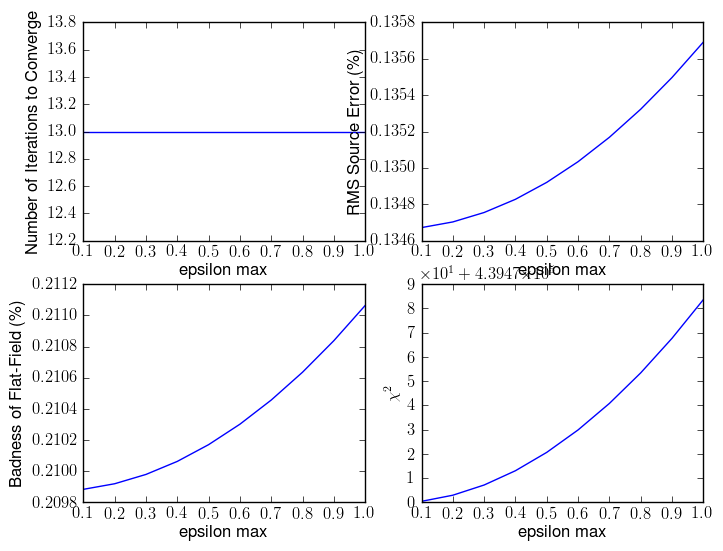
\includegraphics[width=\textwidth]{epsilon_max.png}
\end{center}
\end{figure}


\begin{figure}[ht]
\begin{center}
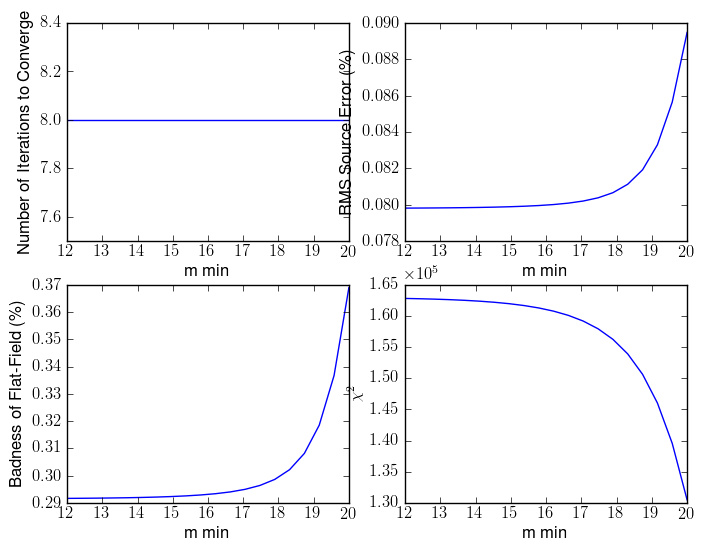
\includegraphics[width=\textwidth]{m_min.png}
\end{center}
\end{figure}

\begin{figure}[ht]
\begin{center}
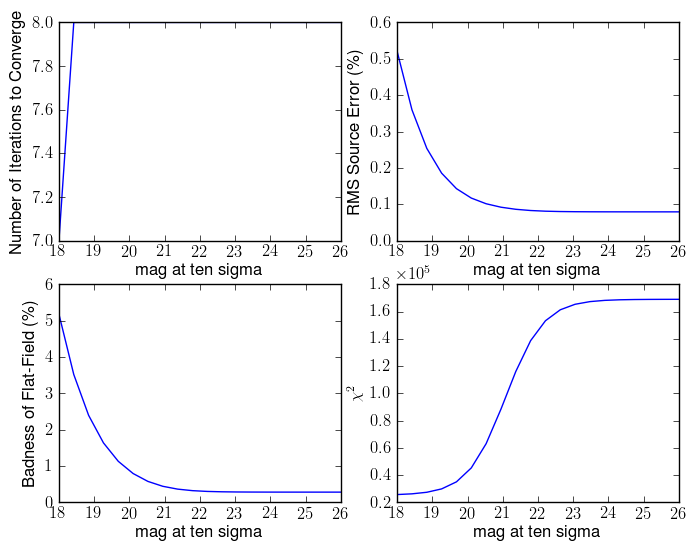
\includegraphics[width=\textwidth]{mag_at_10_sigma.png}
\end{center}
\end{figure}

\end{document}



%The following displaymath is used to generate random star magnitudes with the appropriate probability density distribution function:
%
%\begin{displaymath}
%m = \frac{1}{b} \log_{10}{(\left[ 10^{b m_{max}} - 10^{b m_{min}} \right] r + 10^{b m_{min}})}
%\end{displaymath}
%
%\noindent{}where $r$ is a random number in the range [0.0, 1.0). The catalog is shown in Fig. \ref{fig:sky}. 
